% !TeX spellcheck = en_US
\documentclass[11pt,a4paper]{article}
\usepackage[utf8]{inputenc}
\usepackage{amsmath}
\usepackage{amsfonts}
\usepackage{amssymb}
\usepackage{graphicx}
\usepackage{mathtools}
\usepackage[hidelinks]{hyperref}  % most people dont know of this :3

\usepackage{subfig}
\usepackage[margin=0.7in]{geometry}

% \usepackage[backend=bibtex,style=verbose-ibid]{biblatex}
% \addbibresource{citations.bib}

\usepackage{listings}
\usepackage{color}
\definecolor{dkgreen}{rgb}{0,0.6,0}
\definecolor{gray}{rgb}{0.5,0.5,0.5}
\definecolor{mauve}{rgb}{0.58,0,0.82}

\lstset{frame=tb,
  language=Python,
  aboveskip=3mm,
  belowskip=3mm,
  showstringspaces=false,
  columns=flexible,
  basicstyle={\small\ttfamily},
  numbers=none,
  numberstyle=\tiny\color{gray},
  keywordstyle=\color{blue},
  commentstyle=\color{dkgreen},
  stringstyle=\color{mauve},
  breaklines=true,
  breakatwhitespace=true,
  tabsize=3
}


\newcommand{\inv}{^{\raisebox{.2em}{$\scriptscriptstyle-1$}}}
\newcommand{\qed}{\hfill $\blacksquare$}

\newcommand{\integers}{\mathbb{Z}}
\newcommand{\rationals}{\mathbb{Q}}
\newcommand{\reals}{\mathbb{R}}
\newcommand{\complexes}{\mathbb{C}}
\newcommand{\field}{\mathbb{F}}

\author{Jacob Bruner}
\title{Bivariate Statistics Exploration}
\date{\today}

\begin{document}
\maketitle
% \tableofcontents

% \pagebreak

\iffalse
############
heres an example of a code block
\begin{lstlisting}
        def intervalValues(z, n):
            return output # return the sequence of values
\end{lstlisting}

heres an example of an image
\begin{figure}[h]
\begin{center}
\includegraphics[scale=.37]{onefifteen} 
\caption{Sequences Generated by n = 1-15 on Argand Diagram}
\end{center}
\end{figure}
############
\fi

\section{Mean of X, Y for Datasets}
\subsection{Method}
The mean is a commonly used measure of center for a given statistic. To calculate the mean, we can use the following formula: for a given indexed set of values, the mean is written:
\[
\bar{x} = \frac{1}{N} \sum_{i = 1}^{N} x_i
\]
Where N is the length of the data set. In other words, the mean is the sum of each value divided by the number of values for a given parameter. \\


Calculating these values for each dataset we obtain:

\begin{figure}[ht]
\centering
\begin{tabular}{|l|cc|cc|cc|cc|}
\hline
\textbf{Data set}         & \multicolumn{2}{c|}{\textbf{I}}              & \multicolumn{2}{c|}{\textbf{II}}             & \multicolumn{2}{c|}{\textbf{III}}            & \multicolumn{2}{c|}{\textbf{IV}}             \\ \hline
\textbf{Parameter} & \multicolumn{1}{c|}{\textit{x}} & \textit{y} & \multicolumn{1}{c|}{\textit{x}} & \textit{y} & \multicolumn{1}{c|}{\textit{x}} & \textit{y} & \multicolumn{1}{c|}{\textit{x}} & \textit{y} \\ \hline
\textbf{Mean}     & \multicolumn{1}{c|}{9.0}        & 7.5        & \multicolumn{1}{c|}{9.0}        & 7.5        & \multicolumn{1}{c|}{9.0}        & 7.5        & \multicolumn{1}{c|}{9.0}        & 7.5        \\ \hline
\end{tabular}
\end{figure}

\subsection{Interpretation}

After computing the mean for each, it's clear that the means for each $x, y$ of the respective datasets are equal. Without any other prior knowledge, one might infer that these datasets have a similar center, save variation or spread. This is because the mean doesn't provide information about the variation or spread of the data. Despite this, however, one might assume it to be a reasonable assumption that these datasets and parameters might be highly similar, especially because they match in two variables.

\section{Exploring Other Statistical Measures}

In addition to computing the mean, there are a number of other tools that provide insight into the properties of a dataset. For instance, the variance and standard deviation convey a measure of the 'spread' or variation in a dataset. Similarly, 'Peterson's Correlation Coefficient' often denoted with its square, $r^2$, is meaasure of the \textit{linear} coorelation of two parameters. Values of $r$ range from -1 to 1, with numbers farther from zero denoting stronger coorelation. A closely related notion is the covarience, which measures the linear coorelation, but with a magnitude not necessarily between $(-1, 1)$. These measures are related like so: $r = \frac{cov(x, y)}{\sigma_x \sigma_y}$ where $\sigma$ denotes the standard deviation.

\begin{figure}[]
\centering
\begin{tabular}{l|c|c|c|c|c|c|c|c|}
\cline{2-9}
                                     & \textbf{$\bar{x}$} & \textbf{$\bar{y}$} & \textbf{$\sigma_x^2$} & \textbf{$\sigma_y^2$} & \textbf{$\sigma_x$} & \textbf{$\sigma_y$} & \textbf{$r^2$} & \textbf{$cov(x, y)$} \\ \hline
\multicolumn{1}{|l|}{\textbf{set 1}} & 9.0                & 7.5              & 11.0                & 4.13                & 3.32                  & 2.03                  & 0.67           & 5.5                  \\ \hline
\multicolumn{1}{|l|}{\textbf{set 2}} & 9.0                & 7.5              & 11.0                & 4.13                & 3.32                  & 2.03                  & 0.67           & 5.5                  \\ \hline
\multicolumn{1}{|l|}{\textbf{set 3}} & 9.0                & 7.5              & 11.0                & 4.12                & 3.32                  & 2.03                  & 0.67           & 5.5                  \\ \hline
\multicolumn{1}{|l|}{\textbf{set 4}} & 9.0                & 7.5              & 11.0                & 4.12                & 3.32                  & 2.03                  & 0.67           & 5.5                  \\ \hline
\end{tabular}
\end{figure}

\section{Plots}

Using the python packages \texttt{matplotlib} and \texttt{numpy}, we can plot each dataset like so:

\begin{lstlisting}
for i in range(4):
  dfs[i].plot.scatter(x='x', y='y') 
  reg = np.polyfit(dfs[i]['x'], dfs[i]['y'], 1)
  rval = stats.pearsonr(dfs[i]['x'], dfs[i]['y'])[0]
  plt.plot(dfs[i]['x'], np.polyval(reg, dfs[i]['x']), 'r', label='y={:.2f}x+{:.2f}\n r^2 = {:.2f}'.format(reg[0], reg[1], rval**2))
  plt.xlabel('X')
  plt.ylabel('Y')
  plt.legend()
  plt.savefig('dataset{}.png'.format(i+1))
\end{lstlisting}

After doing so, we get the following interesting results:

\begin{figure}[htbp]
\centering
\subfloat[Dataset I]{\label{fig:a}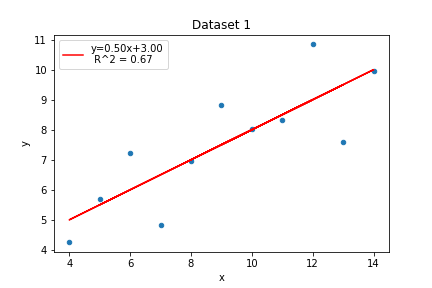
\includegraphics[width=0.45\linewidth]{dataset1.png}}\qquad
\subfloat[Dataset II]{\label{fig:b}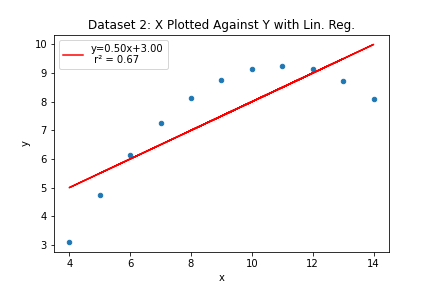
\includegraphics[width=0.45\linewidth]{dataset2.png}}\\
\subfloat[Dataset III]{\label{fig:c}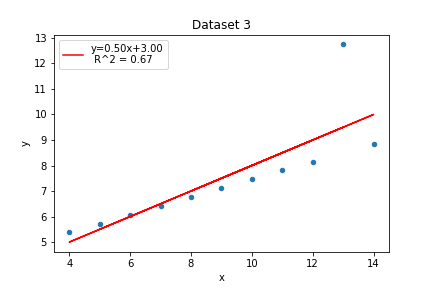
\includegraphics[width=0.45\textwidth]{dataset3.png}}\qquad%
\subfloat[Dataset IV]{\label{fig:d}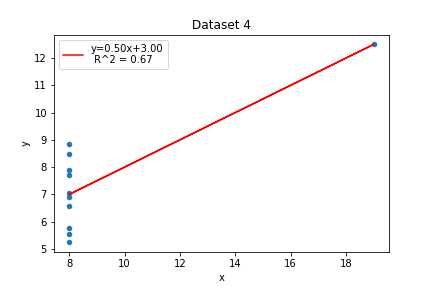
\includegraphics[width=0.45\textwidth]{dataset4.png}}%
\caption{Plot of Datasets I-IV — X against Y with Lin. Reg.}
\label{fig:myfig}
\end{figure}

\end{document}